
\section{Auswertung von Messvergleichen mit Referenzlabor}
In dieser Vorlesung wird die Anwendung des t-Tests und des Chi2-Tests auf eines der zentralen Themen der Metrologie gezeigt, 
welches die Durchführung von Ringvergleichen ist. Wesen der Metrologie ist, dass Messgrößen auf die SI-Einheiten zurückgeführt werden, 
damit sie weltweit vergleichbar sind. Um die Vergleichbarkeit von Ergebnissen unterschiedlicher gesetzlich geprüfter Laboratorien, seien dies Staatsinstitute verschiedener Länder oder Kalibrierlaboratorien innerhalb eines Landes, zu gewährleisten, werden Ringvergleiche durchgeführt.
Dazu wird beispielsweise ein Messobjekt (Prüfkörper) rumgeschickt und jedes beteiligte Labor misst an demselben Objekt eine genau spezifizierte Messgröße nach einem vorgegebenen Verfahren. Um die Ergebnisse miteinander zu vergleichen, werden die statistischen Verfahren der Hypothesentests auf Gleichheit der Mittelwerte und der Standardabweichungen eingesetzt.

Es wird bei der Verwendung des t-Tests danach unterschieden, ob die Nullhypothese getestet wird, dass Mittelwerte der Laboratorien mit einem Erwartungswert (dem Referenzwert) übereinstimmen.
Der Referenzwert wird beispielsweise von einem Referenzlabor zur Verfügung gestellt, das die Möglichkeit hatte, mit deutlich mehr Aufwand und genaueren Geräten, messen zu können.
Für den Vergleich wird die zu vergleichende Messgröße normiert, wie wir es in der letzen Vorlesung schon kennengelernt hatten.

Wir betrachten die Messergebnisse mit Größenwerten $x_i$ für $i = 1,\dots,N$ und Unsicherheiten $u_i$ von $N$ Laboratorien (Partner des Ringvergleichs).

Die standardnormalverteilen Zufallsgrößen, die die Differenz zwischen dem Ergebnis eines Labors bezogen auf den Referenzwert repräsentieren, werden auch Z-Scores oder Z-Werte genannt. Sie werden genutzt, wenn z.~B. das Messergebnis eines
Partners $i$ mit dem Referenzwert (Erwartungswert) verglichen werden soll.
Liegt das Messergebnis des Partners $i$ oberhalb des Referenzwertes, so ist der Z-Wert positiv.
Liegt das Messergebnis  unterhalb des Erwartungswertes, so ist der Z-Wert negativ. 
Um den Z-Wert zu bestimmen, müssen der Erwartungswert $\mu$ und die 
Standardabweichung $\sigma$ der zu Grunde liegenden Verteilung 
bekannt sein. Es reicht nicht aus nur die empirischen Werte (empirischer Erwartungswert, d.h.\
Mittelwert, und empirische Standardabweichung) aus den Stichproben zu schätzen.
Ist $X$ eine Zufallsvariable mit dem Erwartungswert $\mathrm{E}(X)=\mu$ und 
der Varianz $\mathrm{Var}(X) = \sigma^2$ erhält man die zugehörige normierte Zufallsgröße $Z$ durch:
\begin{equation}
Z=\frac{X-\mu}{\sigma}
\end{equation}
Für den Erwartungswert und die Varianz von $Z$ gilt:
\begin{itemize}
	\item $\mathrm{E}(Z) = \mathrm{E}\left( \frac{X-\mu}{\sigma} \right) =
	\frac{1}{\sigma} (\mathrm{E}(X) -\mu) = 0$
	\item $\mathrm{Var}(Z) = \mathrm{Var} \left(\frac{X-\mu}{\sigma} \right) = 
	\mathrm{Var} \left(\frac{X-\mu}{\sigma} \right) = 
	\frac{1}{\sigma^2} \mathrm{Var}(X) = 1$
\end{itemize}

\begin{figure}[!htp]
	\begin{center}
		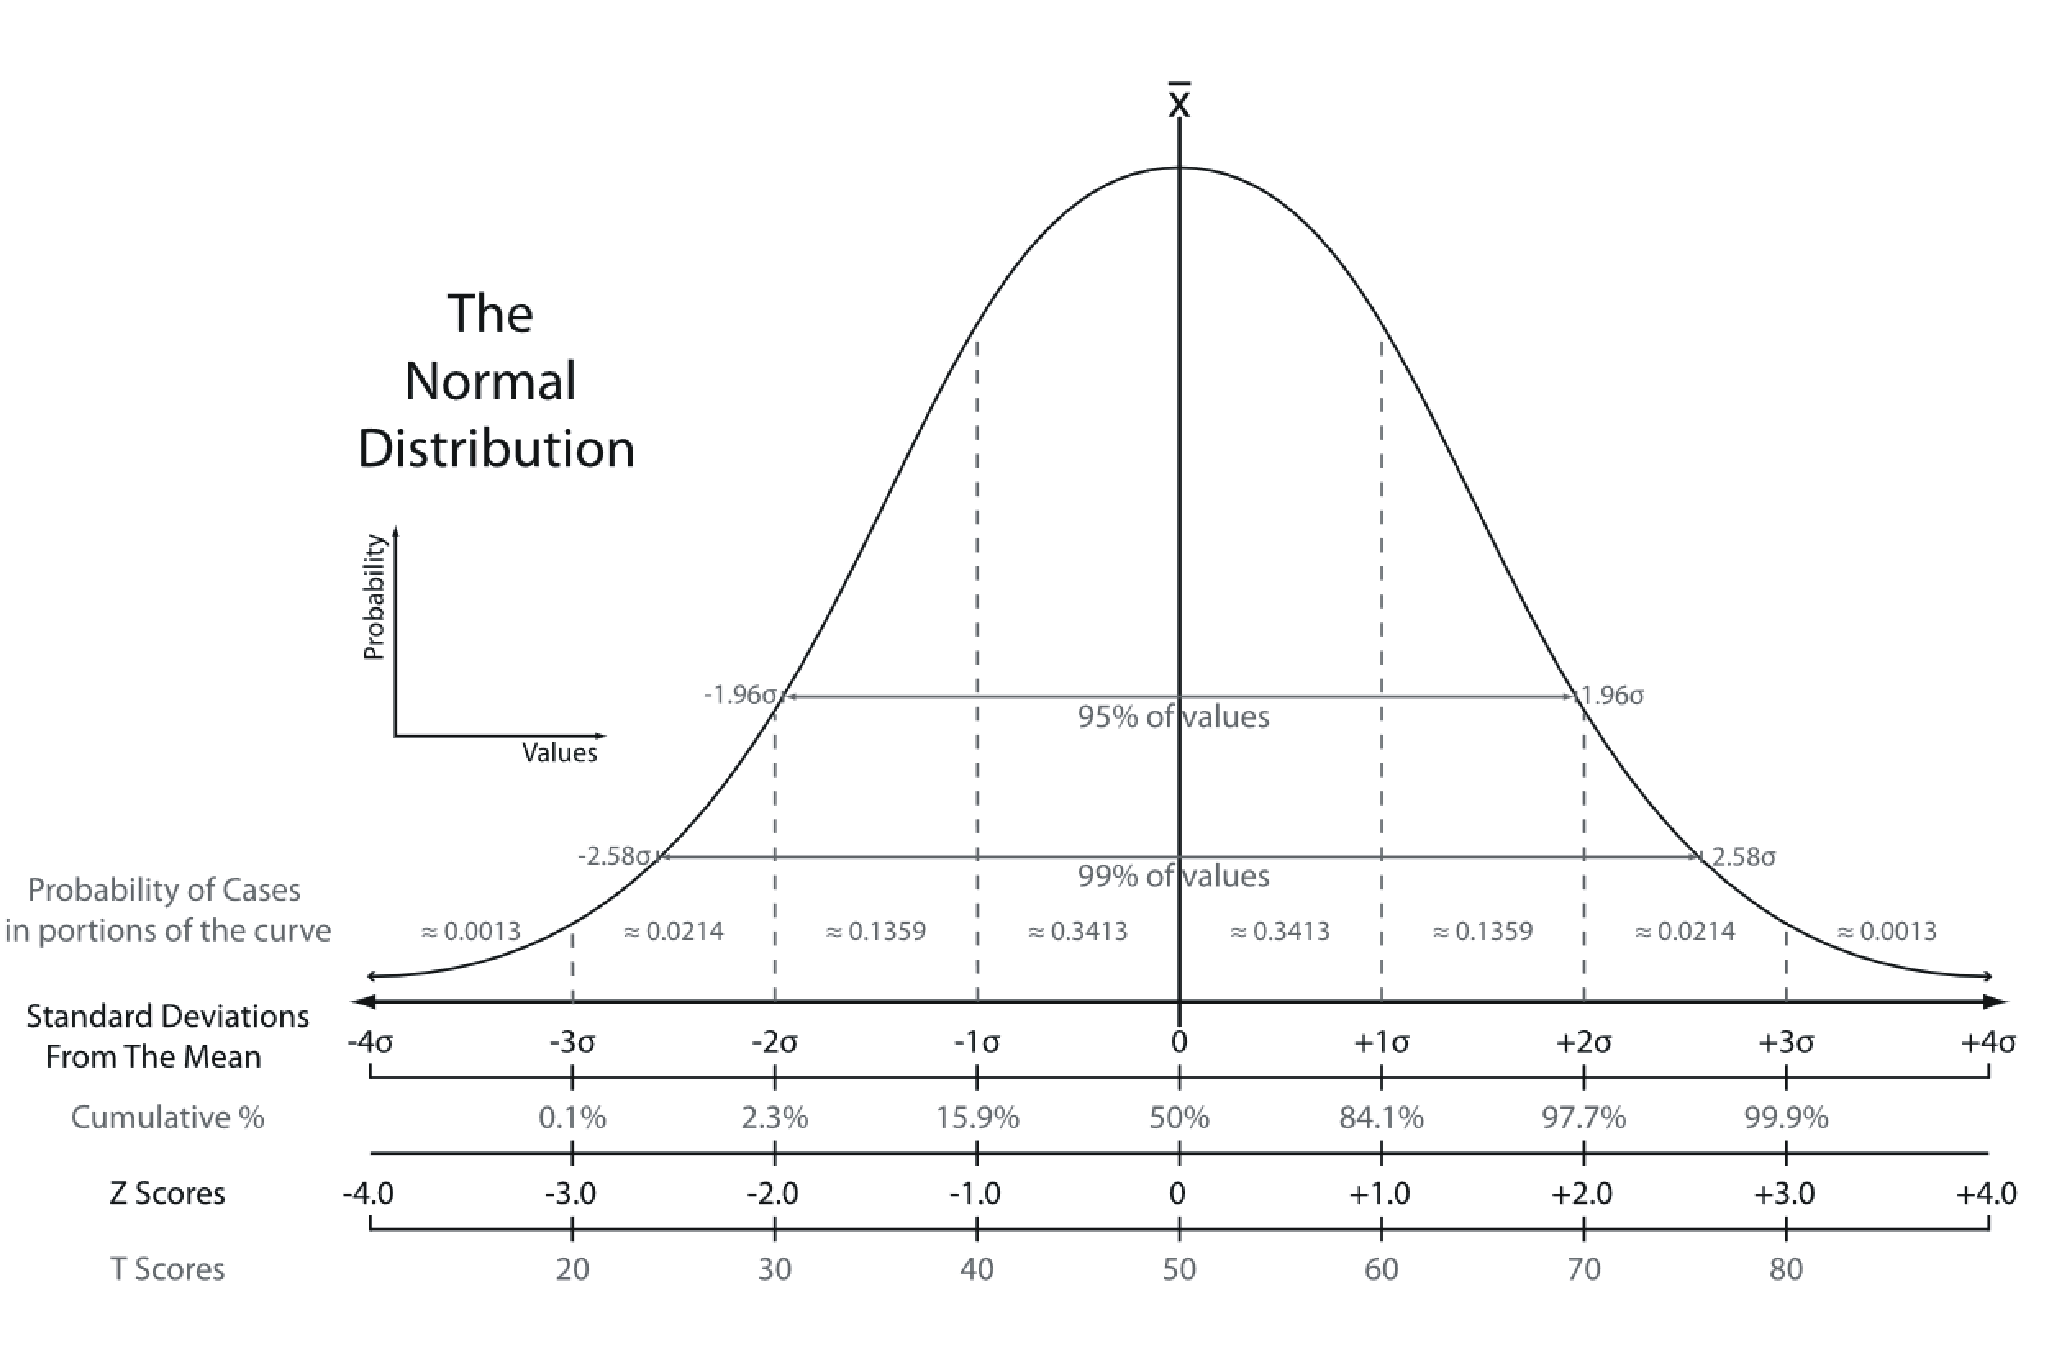
\includegraphics[width=150mm]{06_vorlesung/media/StandardScore.png}
		\caption{Die Standard-Normalverteilung $\mathcal{N}(0,\sigma^2)$ mit den entsprechenden Z-Werten.\newline 
		Quelle: https://en.wikipedia.org/wiki/Standard\_score }
		\label{fig:StandardScore}
	\end{center}
\end{figure}
In Abb.\ref*{fig:StandardScore} ist eine Standardnormalverteilung mit den 
Z-Scores (Z-Werten) dargestellt. 
Z-Scores können nur berechnet werden, wenn die zugrunde liegende Verteilung bekannt ist.
Im Falle von t-Tests haben wir hingegen auch die Möglichkeit auf die aus der Stichproben
geschätzten Parameter für den Erwartungswert und die Varianz zurückzugreifen.
In Abb.\ref*{fig:StandardScore} ist zusätzlich zu der Größe Z-Score ein weitere weitere
Größe aufgetragen: T-Score. Diese ist direkt proportional zu den Z-Scores nur mit einer
anderen Normierung, derart skaliert, dass ihr Erwartungswert $50$ ist und die
Standardabweichung den Wert $10$ annimmt. 

Entsprechend der internationalen Norm \cite{ISO13528} kann der Z-Wert für den Vergleich eines 
Messwertes $x_{i}$ eines Labors~$i$ mit dem Referenzwert $x_\mathrm{ref}$, der eine
Standardabweichung (Standardunsicherheit) $\sigma_\mathrm{ref}$ hat, verglichen werden.
Es wird folgender Z-Score berechnet und anschließend bewertet: 
\begin{equation}
 z_i = \frac{x_{i}-x_\mathrm{ref}}{\sigma_\mathrm{ref}}
\end{equation}
Nach \cite{ISO13528} gibt es die folgende übliche Interpretation für die Bewertung: 
\begin{itemize}
	\item Ein Ergebnis mit $|z_i| \le 2.0$ ist noch akzeptabel.
	\item Ein Ergebnis mit $ 2.0 < |z_i| < 3.0$ gibt ein Warnsignal.
	\item Ein Ergebnis mit $|z_i| \ge 3.0 $ wird als nicht akzeptierbar bewertet. 
\end{itemize}
Sind die erweiterten Unsicherheiten sowohl des Referenzlabors $U_\mathrm{ref}$ als auch 
des Teilnehmerlabors des $i$-ten Partners $U_{i}$ für das % 95,45\% 
Überdeckungsintervall $[-1,\!96 u; 1,\!96 u]$ zum 97,5\% Vertrauensniveau bekannt,
so kann der sogenannte \textbf{En-Wert} berechnet werden. 

In der vorigen Vorlesung hatten wir die Prüfgröße 
$T = \frac{x_1 - x_2}{\sqrt{s_1^2 + s_2^2}}$, die prüft ob zwei Stichproben mit ihren Erwartungswerten
$x_1$ und $x_2$ zur selben Grundgesamtheit gehören.
Dieser Hypothesentest prüft diese Größe auf $|T| > k$. Der Parameter $k$ steht hier allgemein für das Quantil,
also für $z_{1-\alpha/2}$ im Falle der Verwendung der Standardnormalverteilung wie sie hier in Abb.~\ref{fig:StandardScore}
dargestellt ist. Er steht für das Quantil $t_{1-\alpha/2,\nu}$ im Falle der Verwendung der t-Verteilung ($\alpha$: Signifikanzniveau, $\nu$:
Freiheitsgrad). Ferner steht der Parameter $k$ auch für das Quantil einer Posteriorverteilung, also den Faktor
eines \textsl{Credible} Intervalls, weshalb er allgemein \textsl{Erweiterungsfaktor} genannt wird.

Wenn wir eine Unsicherheit $u_i$ eines Labors vorliegen haben, die beispielsweise eine Standardabweichung $s_i$ sein kann, und haben wir ein symmetrisches Überdeckungsintervall, wie es bei normalverteilten oder t-verteilten Zufallsgrößen der Fall ist, so ist die halbe Breite des Überdeckungsintervalls $U_i = k u_i$. Dabei wird $U_i$ die \textsl{erweiterte Messunsicherheit} genannt.

Jetzt dividieren wir die Prüfgröße $T$ durch das Quantil bzw. den Erweiterungsfaktor $k$
$$
\frac{T}{k} = \frac{x_1 - x_2}{k \sqrt{s_1^2 + s_2^2}}  = \frac{x_1 - x_2}
{\sqrt{(k s_1)^2 + (k s_2)^2}} 
$$
und führen die bei Ringvergleichen allgemein verwendete Bezeichnung $E_n := T /k$ ein,
so dass die Prüfgröße mit $U_i = k u_i$ bzw.\  $U_i = k s_i$ wie folgt aussieht:
\begin{equation}
E_\mathrm{n} = \frac{x_{i}- x_\mathrm{ref}}{\sqrt{U_{i}^2+U_\mathrm{ref}^2}}
\label{eq:EnWert}
\end{equation}
Der \textbf{En-Wert} gibt an, wie gut der Laborwert $x_{i}$ mit dem 
Referenzwert $x_\mathrm{ref}$ übereinstimmt. Es werden hier die erweiterten Messunsicherheiten $U$ für $k=2$ kombiniert.
Da hier mit den erweiterten Unsicherheiten gerechnet wird, liegen die Grenzen der akzeptablen Werte nicht bei 2 sondern bei 1.
$|E_n|$ ist gemäß t-Test zu bewerten (siehe auch \cite{ISO13528}):
\begin{itemize}
	\item $|E_\mathrm{n}| < 1$: Die Nullhypothese wird angenommen und gilt als Indikator für eine gute Übereinstimmung
	\item $|E_\mathrm{n}| \ge 1$: Die Nullhypothese wird abgelehnt und gilt als Indikator, dass die Messdaten nicht konsistent zueinander sind.
\end{itemize} 

\section{Auswertung von Ringvergleichen ohne Referenzlabor}
\subsection{Vorgehensweise}
Ringvergleiche zwischen den NMIs (\textsl{National Metrology Institutes}), sog. 
\textbf{Key-Com\-pari\-sons} dienen u.a. dazu einen Referenzwert (KCRV: \textsl{key comparison reference
value}) mit einer zugeordneten Unsicherheit festzulegen.
Der Grad der Übereinstimmung der Messdaten von teilnehmenden Instituts $i$ zum Referenzwert ist hier gesucht. Es gibt keinen Referenzwert, weil man a priori nicht davon ausgehen kann, dass es ein Staatsinstitut gibt, das signifikant besser messen kann als alle anderen.
Ein mögliches Auswerteverfahren, das häufig Anwendung findet, ist bei 
\cite{Cox02} beschrieben. Bei diesem Auswerteverfahren müssen 
folgende 3 Voraussetzungen erfüllt sein: 
\begin{itemize}
	\item Jeder teilnehmende Partner $i$ ($i=1, \dots, N$) stellt Messdaten $x_i$ mit 
	beigeordneter Messunsicherheit $u(x_i)$ eines Prüflings bereit. Der 
	Prüfling muss eine gute Stabilität - auch während des Transportes -
	aufweisen. 
	\item Jeder Partner stellt Messdaten zur Verfügung, die 
	unabhängig von den anderen Partnern sind. D.h. es darf keine 
	Messung eines Partners $i$ von einem anderen Partner $j$ mit $i \ne j$ abhängen. 
	\item Die Messdaten jedes Partners (Instituts) sind normalverteilt.
\end{itemize}

Gegeben sind $N$ teilnehmende Institutionen mit $i=1,\dots,N$. Jeder
Partner/Institut $i$ stellt ein Messergebnis der Messgröße zur Verfügung, also einen Schätzwert $x_i$ und eine zugeordnete Standardmessunsicherheit
$u(x_i)$.
Der Ablauf der Auswertung sieht wie folgt aus:
\begin{itemize}
\item \textbf{Schritt 1:}  \newline
Da kein Referenzwert vorliegt, wird in diesem Fall ein gewichteter Mittelwert $\tilde x$ aus den Messergebnissen aller Partner bestimmt. Benutze dazu das inverse der Quadrate der zugeordneten Standardmessunsicherheiten als Gewichte: 
\begin{equation}
\tilde x = \frac{x_1/u^2(x_1)+ \cdots + x_N/u^2(x_N)}{1/u^2(x_1)+ \cdots 1/u^2(x_N)} = \frac{\sum\limits_{i=1}^{N} x_i / u^2(x_i)}
{\sum\limits_{i=1}^{N} u^{-2}(x_i)}
\label{eq:referenzgleichepartner}
\end{equation}
\item \textbf{Schritt 2:}  \newline
Bestimme die Standardabweichung des gewichteten Mittelwertes $u(\tilde x)=\sigma(\tilde x)$:
\begin{equation}
\frac{1}{u^2(\tilde x)} = \frac{1}{u^2(x_1)} +\cdots + \frac{1}{u^2(x_N)}
\label{eq:Standardabweichung_Mittelwert}
\end{equation}
\item \textbf{Schritt 3:}  \newline
Führe einen Konsistenzcheck durch, ob die angegeben Messergebnisse
konsistent zueinander sind. Führe dazu den $\chi^2$-Test
durch mit der $\chi^2$-Variablen (Testgröße $T$): 
\begin{equation}
T := \chi^2_\mathrm{obs} = \frac{(x_1 - \tilde x)^2}{u^2(x_1)} + \cdots + 
\frac{(x_n-\tilde x)^2}{u^2(x_N)}
\label{eq:T_for_consistencecheck}
\end{equation}
Diese Testgröße weist eher einen kleinen Wert auf, wenn alle Partner 
recht dicht am Mittelpartner liegen und natürlich umgekehrt. 
Vergleiche diese Testgröße mit der $\chi^2 (\nu)$ -Verteilung 
mit Freiheitsgrad $\nu = N-1$ ($N$ Anzahl der Partner), 
die am Messvergleich teilgenommen haben. 
Der Konsistenzcheck schlägt fehl, wenn die folgende Bedingung
erfüllt ist: 
\begin{equation}
\mathrm{Pr}\left(\chi^2(\nu) > T\right) < 0.05
\label{eq:consistencecheck}
\end{equation}
\glqq Pr\grqq~steht für \glqq Probability (Wahrscheinlichkeit)\grqq.
Der $\chi^2$-Test verlangt als Voraussetzung, dass die Messergebnisse
normalverteilt sind. 

\item \textbf{Schritt 4:}  \newline
Falls der Konsistenzcheck nicht fehlschlägt, wird der Wert $\tilde x$ als
Referenzwert (KCRV: key comparison reference value) $x_\mathrm{ref}$ akzeptiert
mit der Unsicherheit $u(x_\mathrm{ref}) = u(\tilde x)$. Nun kann der \textbf{Grad 
der Übereinstimmung} $d_i = x_i - x_\mathrm{ref}$ der Partner $i=1,\dots, N$ mit dem Referenzwert $x_\mathrm{ref}$ wie folgt bestimmt werden. 
Wir definieren die normierten Gewichte $\tilde w_i$
\begin{equation}
\tilde w_i := \frac{u^2(x_\mathrm{ref})}{u^2(x_i)}
\label{eq:anteile}
\end{equation}
mit
\begin{equation}
\sum_{i=1}^{N} \tilde w_i = 1 .
\label{eq:normierung}
\end{equation}
Der Referenzwert $x_\mathrm{ref} \equiv \tilde x$ aus Gl.~(\ref{eq:referenzgleichepartner}) sie damit wie folgt aus: 
\begin{equation}
x_\mathrm{ref} = \sum_{i=1}^{N} \tilde w_i\; x_i
\label{eq:referenzgleichepartner2}
\end{equation}

Für den Grad der Übereinstimmung erhalten wir: 
\begin{equation}
d_i = x_i - x_\mathrm{ref} = x_i - \sum_{j=1}^{N} \tilde w_j x_j 
= x_i - \tilde w_i x_i - \sum_{\substack{j=1 \\ j \neq i}}^{N} \tilde w_j x_j 
= (1-\tilde w_i)x_i - \sum_{\substack{j=1 \\ j \neq i}}^{N} \tilde w_j x_j 
\end{equation}
Wenn die Messungen nicht gegenseitig voneinander abhängen, so kann 
zur Berechnung der Unsicherheit von $d_i$ das Gesetz der Fortpflanzung
der Unsicherheiten angewendet werden. (Hinweis: Sind ein Modell mit $y=f(x_1, x_2)$ und 
die dazugehören Unsicherheiten $u(x_1)$ sowie $u_(x_2)$ gegeben, so ergibt sich die Unsicherheit von
$y$ bei Nichtkorrelation von $x_1$ und $x_2$ nach dem Gesetz der Fehlerfortpflanzung zu: 
$u^2(y)=\left(\frac{\partial f}{\partial x_1}\right)u^2(x_1)+\left(\frac{\partial f}{\partial x_2}\right)u^2(x_2)$)

Für die Unsicherheit der Differenz $d_i$ ergibt sich somit:
\begin{eqnarray}
u^2(d_i) &=& \left( \frac{\partial d_i}{\partial x_i} \right)^2 \cdot u^2(x_i) +  \sum_{\substack{j=1 \\ j \neq i}}^{N}
\left( \frac{\partial d_i}{\partial x_j} \right)^2 \cdot u^2(x_j) \\
&=&  (1-\tilde w_i)^2 u^2(x_i) + \sum_{\substack{j=1 \\ j \neq i}}^{N} \tilde w_j^2 u^2( x_j) \\
&=& ((1-\tilde w_i^2)-\tilde w_i^2)u^2(x_i) + \sum_{j=1}^{N} \tilde w_j^2 u^2(x_j) 
\end{eqnarray}
Mit Gl.(\ref{eq:anteile}) ergibt sich:
\begin{equation}
u^2(d_i) = (1-2\tilde w_i^2)u^2(x_i) + \sum_{j=1}^{N} \tilde w_j u^2(x_\mathrm{ref}) 
\end{equation}
Mit Gl.(\ref{eq:anteile}) und Gl.(\ref{eq:normierung}) ergibt sich daraus:
\begin{eqnarray}
u^2(d_i) &=& u^2(x_i) - 2u^2(x_\mathrm{ref}) + u^2(x_\mathrm{ref}) \sum_{j=1}^{N}\tilde w_j  
\nonumber \\
  &=& u^2(x_i) -u^2(x_\mathrm{ref})
\end{eqnarray}
Auch hier kann nun wieder ein En-Wert angeben werden. Da alle Größen normalverteilt sind, sind die erweiterten Unsicherheiten für einen 
Erweiterungsfaktor von $k=2$, $U(x_i) = k \cdot u(x_i) =2 \cdot u(x_i)$. Damit lässt sich der En-Wert mit Gl.(\ref{eq:EnWert}) bestimmen, der den
Grad der Übereinstimmung des beteiligten Partners $i$ mit dem Referenzwert
angibt.
\begin{equation}
E_\mathrm{n}(x_i) = \frac{d_i}{2\sqrt{u^2(d_i)}}
\end{equation}
\end{itemize}

Es gelten wieder die Aussagen von Kapitel 1:
\begin{itemize}
	\item $|E_\mathrm{n}| < 1$ ist ein Indikator für eine gute Übereinstimmung.
	\item $|E_\mathrm{n}| \ge 1 $ ist ein Indikator, dass die Messdaten nicht konsistent zueinander sind.
\end{itemize} 
\subsection{Beispiel}
\label{Beispielringvergleich1}
% \textbf{Beispiel} \newline
5 Partner messen ein Massestück von ca. 100 g. Die Ergebnisse 
der Partner sind wie folgt (alle Angaben sind in g):
\begin{center}
\begin{tabular}{l | c c c c c}
$i$	& 1 & 2 & 3 & 4 & 5 \\	\hline
$x_i / \mathrm{g}$ & 99.82 &  99.05 & 99.17 & 99.20 & 99.38  \\ \hline
$u(x_i) / \mathrm{g}$ & 0.80 & 0.63 & 0.86 & 0.82 & 0.98  
\end{tabular}
\end{center}
Als Ergebnis erhalten wir: $x_\mathrm{ref} = 99.29$ und $u_\mathrm{ref} = 0.35$. 
Mit der Testgröße $T=0.6239$ ergibt sich die Wahrscheinlichkeit 
$\mathrm{Pr}\{\chi^2(\nu) > T\} = 0.8858$. Da die Wahrscheinlichkeit größer als 0.05 ist, schlägt der
Konsistenzcheck nicht fehl, 
d.h.\ die Daten der 5 Messpartner sind konsistent.

Für die Abweichungen $d_i$ erhalten wir: 
$$
[0.7172 \;\;   0.5209 \;\;   0.7836  \;\;  0.7395 \;\;   0.9137]. 
$$
Für die En-Werte erhalten wir: 
$$
[ 0.3676 \;\;  -0.2329 \;\;  -0.0783 \;\;  -0.0626 \;\;   0.0478].
$$
Das heisst der Partner 5 ist in bester Übereinstimmung mit dem Referenzwert. \\
Der Octave-/Matlab-Code dazu lautet (Hinweis zu Octave: Evtl. ist die Funktion
\texttt{chi2pdf} in Octave noch nicht vorhanden. Dann zuerst das Paket statistics
installieren, \texttt{pkg install -forge package\_name} mit 
\texttt{package\_name = statistics}): 
\begin{verbatim}
% clear all;
x = [99.82, 99.05, 99.17 , 99.20 ,99.38];
u_x = [0.80 0.63, 0.86, 0.82, 0.98];
U_x = 2*u_x;

% Anzahl der Freiheitsgrade
nu = 4;

% Schritt 1:
x_ref = sum(x./(u_x).^2) ./ sum(1./(u_x).^2)

% Schritt 2: 
u_ref = sqrt(1./sum(1./(u_x).^2))

% Schritt 3: 
T = sum((x-x_ref).^2./(u_x.^2))

% Bestimme die Wahrscheinlichkeit Pr der Chi^2-Verteilung für Chi^2(\nu) > T:
Pr = 1 - chi2pdf(T,nu)

% Schritt 4: Grad der Übereinstimmung
d = x-x_ref;
u_d = sqrt(u_x.^2 - u_ref.^2)
En = d./(2*sqrt(u_d.^2))
\end{verbatim}

\subsection{Identifikation von Ausreißern und Konsistenzcheck}
Wir wollen uns hier noch etwas genauer anschauen, wie man feststellt, 
ob die Messdaten eines Ringvergleiches konsistent sind und wie man mit Inkonsistenten umgeht.
Als \textbf{Ausreißer} werden häufig Messwerte deklariert, deren Abweichungen größer  
als 3 mal die erweiterte Messunsicherheit des Referenzwertes \cite{GuideKey} sind.
Diese Ausreißer werden in Abstimmung mit dem Partner gelöscht. 
Anschließend werden die verbliebenen Daten auf statistische Konsistenz
überprüft. Wir haben dazu bereits in Gl.(\ref{eq:T_for_consistencecheck}) und Gl.(\ref{eq:consistencecheck}) 
eine Formel angegeben, mit der überprüft werden kann, ob die angegebenen
Messergebnisse (Messwerte mit Unsicherheiten) konsistent zu dem Referenzwert und 
dessen Unsicherheit ist. Die Testgröße $T$ basiert auf dem Birge-Test, 
welche ebenso ein Test auf die Konsistenz der Messdaten in einem Ringvergleich
ist. Der Birge-Test ist wie der $\chi^2$-Test nur unter folgenden Bedingungen
gültig:
\begin{itemize}
	\item Die gemessenen Messwerte $x_i$ der $N$ Institute sind unkorreliert
	\item Man benötigt Kenntnis über die Verteilungsdichtefunktionen. Es 
	wird vorausgesetzt, dass die Größen normalverteilt mit den Unsicherheiten $u(x_i)$ bzw. den Varianzen $\sigma_i$ sind.
\end{itemize}
Das Birge-Verhältnis ist -bis auf die Anzahl der Freiheitsgrade- die Prüfgröße des Chi2-Tests
(siehe vorherige Vorlesung, Gl.~\ref{chi2testgroesse}).
Es wird folgendes geprüft ($H_0$: Nullhypothese, $H_a$: Alternativhypothese):
\begin{center}
	\begin{tabular}{l | p{14cm} }
	$H_0$	& $u_\mathrm{partner}^2 =  u_\mathrm{ref}^2$:\newline 
	Die Stichprobe gehört zu 
		einer Grundgesamtheit  mit Varianz $u_\mathrm{ref}^2$\\	\hline
 $H_\mathrm{a}$	& $u_\mathrm{partner}^2 \neq  u_\mathrm{ref}^2$: \newline 
 Die Stichprobe gehört nicht zu einer Grundgesamtheit mit Varianz $u_\mathrm{ref}^2$\\ 
	\end{tabular}
\end{center}
 
Das \textbf{Birge-Verhältnis} ist definiert als das Verhältnis der Streuungen der Unsicherheiten aller Partner 
(bezeichnen wir mit $u_\mathrm{partner}$) zu der Unsicherheit des Referenzwertes $u_\mathrm{ref}$. Es wird
analog der Testgröße des $\chi^2$-Tests, $T = \nu \left(\frac{s}{\sigma_0}\right)^2$ Gl.~\ref{chi2testgroesse}, wie
folgt definiert:
\begin{equation}
R_\mathrm{B} := \frac{u_\mathrm{partner}}{u_\mathrm{ref}}
\quad \text{mit} \quad 
\frac{u^2_\mathrm{partner}}{u^2_\mathrm{ref}} \, \propto \, 
\nu \left(\frac{s}{\sigma_0}\right)^2.
\end{equation}
Die Varianz aller $N$ Partner ist wie folgt definiert:
\begin{equation}
u^2_\mathrm{partner} := \frac{\frac{1}{N-1} \sum\limits_{i=1}^{N} w_i \left(x_i-x_\mathrm{ref} \right)^2}
{\sum\limits_{i=1}^{N} w_i} \quad \text{mit} \quad w_i = \frac{1}{u^2(x_i)} .
\end{equation}
Entsprechend Gl.(\ref{eq:Standardabweichung_Mittelwert}) ist die Unsicherheit des Referenzwertes wie folgt gegeben
\begin{equation}
u_\mathrm{ref} = \left(\frac{1}{u^2(x_1)} +  \cdots + \frac{1}{u^2(x_N)} \right)^{-\frac{1}{2}},
\end{equation}
so dass für das Birge-Verhältnis gilt
\begin{equation}
R_\mathrm{B} = \sqrt{\frac{1}{N-1} \; \sum_{i=1}^N \left( \frac{x_i-x_\mathrm{ref}}{u(x_i)} \right)^2 }.
		\label{eq:Birge-Verhaeltnis}
\end{equation}

%Vergleicht man das Birge-Verhältnis mit der Testgröße $T$ in Gl.(\ref{eq:T_for_consistencecheck}) so ergibt sich der Zusammenhang:
%\begin{equation} 
%R_\mathrm{B}^2 = \frac{1}{N-1} \; T
%\end{equation}
Bei dem Konsistenzcheck mit dem Birge-Verhältnis wird untersucht, ob  
\begin{itemize}
	\item $R_\mathrm{B} \le 1$: Konsistenzcheck ok. 
	\item $R_\mathrm{B} > 1$: Konsistenzcheck schlägt fehl.
\end{itemize}
Wenn $R_\mathrm{B} > 1$ ist, bedeutet dies, dass entsprechend Gl.(\ref{eq:Birge-Verhaeltnis}) die Unsicherheiten der Partner 
$u(x_i)$ nicht zu der Unsicherheit des Referenzwertes $u(x_\mathrm{ref})$ passen.
Die gemessenen Daten $x_i$ der Partner sind inkonsistent.
Für unser Beispiel Abschnitt \ref{Beispielringvergleich1} erhalten wir $R_\mathrm{B} = 0.39494$.
Damit schlägt der Birge-Test nicht fehl und die Daten sind 
danach konsistent. Für die Auswertung eines Ringvergleichs ist es empfehlenswert sowohl das Birge-Verhältnis als auch den $\chi^2$-Test
(siehe Gl.(\ref{eq:consistencecheck})) durchzuführen und zu prüfen, ob beide Tests ok sind. 

Häufig wird das Birge-Verhältnis in Gl.(\ref{eq:Birge-Verhaeltnis}) 
umgeschrieben und in folgender Form dargestellt:
\begin{equation}
R_\mathrm{B}^2 = \sum_{i=1}^N \frac{w_i (x_i - x_\mathrm{ref})^2}{N-1}
\end{equation}
mit den Gewichten $w_i = 1/\sigma_i^2$ für $i=1,2,\ldots, N$ und dem 
Referenzwert (gewichteten Mittelwert) $x_{ref}=\sum_i w_i x_i / \sum_i w_i$.
Der Birge Test kann auch bei korrelierten Messdaten $x_1,\ldots ,x_N$, wenn die 
Kovarianzen $\sigma_{12},\ldots, \sigma_{(N-1)N}$ gegeben sind, durchgeführt werden, siehe \cite{Kac08}.

\subsection{Paule-Mandel Metjode zur Anpassung von Gewichtsfaktoren}

Bei Ringvergleichen kommt es oftmals vor, dass jeder am Vergleich beteiligte Partner eine
Unsicherheit $U$ angibt die kleiner ist als der Abstand des Messwertes zu anderen Partnern,
so dass der En-Wert bzw.\ des Birge-Verhältnisses unter Verwendung der Gewichte gemäß Gl.~(\ref{eq:anteile})
größer als Eins wird. Durch eine Anpassung der Gewichtsfaktoren durch Hinzufügen einer
zusätzlichen Komponente, die sich aus der Streuung der Ergebnisse von Partner zu Partner ergibt,
kann eine bessere Konsistenz erzielt werden.

Der Leitfaden zum Erstellen eines \textsl{Key Comparison Reports}
\cite{GuideKey} empfiehlt als Anpassungsverfahren die \textbf{Paule-Mandel Methode},
bei der die Varianzen durch Additions einer Streuung zwischen Laboratorien
erhöht werden. Dadurch werden die Gewichtsfaktoren $w_i$ verkleinert und damit Referenzwert 
$x_\mathrm{ref}$ so angepasst, so dass das Birge-Verhältnis kleiner als Eins werden kann.
Ein Beispiel dazu ist im Anhang B der Richtlinie für Ringvergleiche \cite{GuideKey} zu finden.

Im folgenden schauen wir uns das Prinzip von Mandel und Paule an, das 
in der Publikation \cite{Pau82} zu finden. Es werden zwei eher künstliche Beispiele gewählt, um das Prinzip besser zu verstehen. 
In Beispiel I wird eine Messgröße mit zwei verschiedenen Methoden (bzw.\ von zwei verschiedenen Partnern) A und B gemessen.
Die gemessenen Einzelwerte von jedem der beiden Partner sind in Tab. \ref*{tab:Beispiel_I}
angegeben.
\begin{table}[!htb]
	\caption{Messdaten des Beispiels I}
	\begin{center}
	\begin{tabular}{l| rrr |rrr}
		\hline 
		Methode/Partner & \multicolumn{3}{c}{A} \vline & \multicolumn{3}{c}{B} \\ \hline
		Gemessener Wert $x_i$ & 1.1 & 1.9 & 1.5 & 16 & 25 & 3 \\ \hline
	\end{tabular}
\end{center}
\label{tab:Beispiel_I}
\end{table}

Der gleichgewichtete Mittelwert $\bar x_I$ über alle Werte beider Partner gemeinsam ist:
 \begin{equation}
 \bar x_I = \frac{1}{N} \sum_{i=1}^N x_i \, = \frac{1}{6}\left( 1.1 + 1.9 + 1.5 + 16 + 25 + 3 \right) \, \approx \, 8.1
 \end{equation}
 Intuitiv würden wir jedoch sagen, dass wir den Messdaten mit der Methode A
 mehr vertrauen schenken würden, als den Messdaten mit der Methode B, da die 
 Messdaten der Methode A weniger streuen als die Messdaten mit der Methode B.

 Als zweites Beispiel betrachten wir, dass die Methoden (bzw. Partner) A und B ähnlich
 genau messen, jedoch werden von Partner A einen größeren Stichprobenumfang
 als von Partner B:

 
 \begin{table}[!htb]
 	\caption{Messdaten des Beispiels II}
 	\begin{center}
 		\begin{tabular}{l| rrrrrr |rr}
 			\hline 
 			Methode/Partner & \multicolumn{6}{c}{A} \vline & \multicolumn{2}{c}{B} \\ \hline
 			Gemessener Wert $x_i$ & 2.0 & 1.0 & 1.5 & 1.8 & 1.2 & 1.7 
 			& 16.3 & 16.8\\ \hline
 		\end{tabular}
 	\end{center}
 	\label{tab:Beispiel_II}
 \end{table}
Für den Mittelwert über alle Werte gemeinsam erhalten wir:
 \begin{equation}
 \bar x_{II} = \frac{1}{N} \sum_{i=1}^N x_i \, = \frac{1}{8}\left( 2.0 + 1.0 + 1.5 + 1.8 + 1.2 + 1.7 + 16.3 + 16.8 \right) \, = \, 5.2875
\label{eq:einfachesMittelII}
 \end{equation}
Es fällt auf, dass die beiden Werte von Partner B zueinander passen, sich aber deutlich von denen von Partner A unterscheiden.

Die beiden Mittelwerte der jeweiligen Partner A und B sind
 \begin{equation}
 \bar x_{II,A} = \frac{1}{6}\left( 2.0 + 1.0 + 1.5 + 1.8 + 1.2 + 1.7 \right) = 1.533, 
\quad \bar x_{II,B} = \frac{1}{2}\left( 16.3 + 16.8 \right) = 16.550
 \label{eq:Mittelwerte_x_II_A_B}
 \end{equation}

\textcolor{red}{\textbf{Dieses würde ich hier an dieser Stelle gar nicht bringen, auch wenn es in Pau82 
so präsentiert wird, weil Du ja hier in diesem Skript schon mit den Gewichten als Kehrwert
der Varianzen für den Referenzwert, der aus dem gewichteten Mittel der Resultate aller Partner
gewonnen wurde, um En-Werte für gleiche Partner zu bestimmen.}}


\textcolor{red}{zunächst hatte ich entlang am Pau82 die Sachen so nachgerechnet und verstanden, wie
Paule und Mandel sie argumentiert hatte, dann wurde mir langsam klar, dass wir in unseren Vorlesungen
aber längst an dem Punkt angekommen sind, dass man die Kehrwerte der Varianzen nimmt und nicht
anfängt die Mittelwerte einfach zu mitteln $\Rightarrow$ alles Blaue hiernach hier wegnehmen}

\textcolor{blue}{und der Mittelwert dieser beiden Mittelwerte ist
 \begin{equation}
  \bar x_{II,AB} = \frac{1}{2}\left( 1.533 + 16.550 \right) = 9.0417
 \label{eq:Mittelwerte_x_IIAB}
 \end{equation}
 Dadurch dass wir Mittelwerte mitteln erhalten wir eine andere Wichtung: $\frac{\sum w_i x_i}{\sum w_i}$:
$$
\frac{1}{2} \left( \frac{1}{6} \left(\sum\limits_{i=1}^6 x_i \right) \; + \;
    \frac{1}{2} \left(\sum\limits_{i=7}^8 x_i \right)  \right) =
 \frac{1}{12} \left(\sum\limits_{i=1}^6 x_i \right) \; + \;
    \frac{1}{4} \left(\sum\limits_{i=7}^8 x_i \right)
$$
also 
$$
\frac{w_i}{\sum\limits_{i=1}^8 w_i} \, = \, 
\left\{ \begin{array}{ccl}
\frac{1}{12} & \text{f{\"u}r} & i = 1,\dots,6 \\
\frac{1}{4} & \text{f{\"u}r} & i = 7, 8
\end{array} \right.
$$
Diese Art der Wichtung, die Einzelwerte zu gewichten, führt dazu dass Stichprobe B
sehr viel stärker gewichtet wird, in diesem Beispiel um einen Faktor $3$ mit $\frac{1}{4} = \frac{3}{12}$.
Es macht jedoch mehr Sinn, die Gewichte danach zu richten, wie genau die Größen sind,
im Sinne von der Frage wie breit oder schmal die Wahrscheinlichkeitsdichteverteilung ist.}


Wir haben im Laufe dieser Vorlesungsreihe bereits gesehen, dass
Messergebnisse mit größerer Unsicherheit sinnvollerweise mit geringerer
Wichtung zu berücksichtigen sind, so dass Gewichte
deshalb aus dem Kehrwert der Varianzen bestimmt werden. Der Grund dafür liegt darin,
dass die Varianz des gewichteten Mittelwertes $x_\mathrm{ref}$ minimiert wird,
wenn die Gewichte als Reziprokwert der Varianzen der Einzelwerte berechnet werden.
In Gl.~(\ref{referenzgleichepartner}) bzw.\ Gl.~(\ref{eq:referenzgleichepartner2}) 
haben wir deshalb zur Ermittlung des Referenzwertes $x_\mathrm{ref}$ beim
Ringvergleich mit gleichwertigen Partnern gerechnet mit
\begin{equation*}
    w_i = \frac{1}{u^2_i}
\end{equation*}
und
\begin{equation*}
 x_\mathrm{ref} = \frac{\sum\limits_{i=1}^N w_i x_i}{\sum\limits_{i=1}^N w_i} .
\end{equation*}

\textcolor{red}{wahrscheinlich macht es keinen Sinn mit der empirischen Varianz
anzufangen, sondern direkt mit der empirischen Var des Mittelwertes, also nehme ich
diesen Teil wieder zurück}
\textcolor{blue}{Verwenden wir für die Unsicherheit $u_i$ die empirische Varianz
$u_i = \operatorname{Var}(x_i)$ für Beispiel II folgende Werte
$$
\operatorname{Var}(x_{II,A}) = 
\frac{1}{6-1} \sum\limits_{k=1}^{6} \left(x_{II,k} - \bar x_{II,A} \right)^2 = 0.14267
$$
und
$$
\operatorname{Var}(x_{II,B}) = \frac{1}{2-1} \sum\limits_{k=7}^{8} \left(x_{II,k} - \bar x_{II,B} \right)^2
= 0.12500
$$ 
so erhalten wir für die beiden Gewichte $w_A = 7.0093$ und $w_B = 8.0000$, die beide fast gleich.
Der gewichtete Mittelwert, der als Referenzwert für En-Tests und das Birge-Verhältnis genutzt wird ist damit
$$
x_\mathrm{ref} \; = \; \frac{7.0093 \cdot 1.533 \; + \; 8.0000 \cdot 16.550}{7.0093 + 8.0000}
\; = \; 9.5372
$$
Nach Gl.~(\ref{eq:Birge-Verhaeltnis}) das Birge-Verhältnis hierfür
$$
R^2_\mathrm{B} \; = \; \frac{1}{N-1} \; \sum_{i=1}^N \left( \frac{x_i-x_\mathrm{ref}}{u^2(x_i)} \right)^2 \; = \;
 \frac{1}{2-1} \, \left( \frac{\left(1.5333 - 9.5372\right)^2}{0.14267}
 \, + \, \frac{ \left( 16.550 - 9.5372 \right)^2}{0.12500} \right) = 842.47 \gg 1
$$
--nix!}

Da es sich um den Vergleich der Mittelwerte der beiden Stichproben A und B handelt, verwenden wir
für die Unsicherheit $u_i$ die Varianz des Mittelwertes, also
$u_i = \operatorname{Var}(\bar x_i)$ verwenden. Für Beispiel II sind dies folgende Werte:
$$
\operatorname{Var}(\bar x_{II,A}) = \frac{1}{6(6-1)} \sum\limits_{k=1}^{6} \left(x_{II,k} - \bar x_{II,A} \right)^2 = 0.023778
$$
und
$$
\operatorname{Var}(\bar x_{II,B}) = \frac{1}{2(2-1)} \sum\limits_{k=7}^{8} \left(x_{II,k} - \bar x_{II,B} \right)^2 = 0.062500
\label{eq:VarianzenMWII}
$$
so erhalten wir für die beiden Gewichte $w_A = 42.056$ und $w_B = 16.000$.
Der gewichtete Mittelwert, der als Referenzwert für En-Tests und das Birge-Verhältnis genutzt wird, ist damit
$$
x_\mathrm{ref} \; = \; \frac{42.056 \cdot 1.533 \; + \; 16.000 \cdot 16.550}{42.056 + 16.000}
\; = \; 5.6716
$$
Nach Gl.~(\ref{eq:Birge-Verhaeltnis}) das Birge-Verhältnis hierfür
$$
R^2_\mathrm{B} \; = \; \frac{1}{N-1} \; \sum_{i=1}^N \left( \frac{x_i-x_\mathrm{ref}}{u(x_i)} \right)^2 \; = \;
 \frac{1}{2-1} \, \left( \frac{\left(1.5333 - 5.6716\right)^2}{0.023778}
 \, + \, \frac{ \left( 16.550 - 5.6716 \right)^2}{0.0625} \right) = 2613.7
$$
also
$$
R_\mathrm{B} \; = \; \sqrt{2613.7} \, = \, 51.1  \gg 1
$$

% https://iopscience.iop.org/article/10.1088/0026-1394/51/5/516/meta

Wir sehen, dass die Varianzen der Mittelwerte der beiden Partner A und B im Verhältnis zur
Differenz zwischen den beiden Partnern sehr klein ist, oder umgekehrt gesagt liegen die 
Mittelwerte der Methoden A und B sehr weit auseinander im Verhältnis zu den Varianzen.
Die Varianzen $\operatorname{Var}(\bar x_A)$ und $\operatorname{Var}(\bar x_A)$ beschreiben
nur die interne Streuung, also nur die Streuung der jeweiligen Stichproben A und B.
Die Wahrscheinlichkeitsverteilungen werden durch die beiden Parameter Erwartungswert,
also hier Mittelwert, und Varianz charakterisiert und wir hatten bei den Hypothesentests
gelernt, auf beides zu prüfen. Wir haben gesehen, dass Stichproben einer gemeinsamen
Grundgesamtheit angehören, wenn beides, Mittelwert und Varianz zueinander passen.

Bei den Ringvergleichen, bei denen von verschiedenen Laboratorien oder Instituten mit
unterschiedlichen Methoden oder jedenfalls unabhängigen experimentellen Aufbauten die
Ergebnisse verglichen werden, kann beobachtet werden, dass entweder die
Schätzer (empirischen Erwartungswerte) oder die empirischen Varianzen oder sogar
beides nicht zusammen passen. In der Praxis kommt es vor, dass die jeweiligen
Labore oder Institute ihre Methode immer weiter optimiert haben und ihre Genauigkeit
erhöht haben, dass jedoch verbleibende, unerkannte systematische Effekte vorhanden sind.
Dass es Unterschiede gibt, tritt erst bei dem Vergleich zutage und es lässt sich
im Rahmen der gesetzten Zeit für das Projekt des Vergleichens nicht aufklären.
In solchen Fällen lebt man dann damit, dass es auch zwischen den unterschiedlichen
Methoden bzw.\ Laboren eine Streuung gibt.

Statistisch wird dies damit ausgedrückt, dass die Stichproben auf den verschiedenen
Laboren zu verschiedenen Grundgesamtheiten gehören.
Konkret bedeutet das, dass für die Gewichte zusätzlich zur Varianz des Mittelwert
zur jeweiligen Methode/ des jeweiligen Laboratoriums
(Streuung innerhalb einer Gruppe, \textsl{within group variability})
auch eine Varianz der Methoden/Laboratorien (Streuung zwischen Gruppen,
\textsl{between group variability}) eingeführt.
Die Streuung zwischen den Gruppen, die Varianz $s^2_\mathrm{b}$ wird
iterativ geschätzt. Für die verschiedenen Partner oder Stichproben $A$ und $B$
verwenden wir jetzt die Notation $S_i$, hier also $S_1 = A$ und $S_2 = B$, um
die Gleichungen allgemein aufschreiben zu können.
\begin{equation*}
\operatorname{Var}(\bar x_{S_i,\mathrm{c}}) \; = \;
\operatorname{Var}(\bar x_{S_i}) \; + \; s^2_\mathrm{b} \; = \;
\frac{1}{M_i (M_i - 1)} \sum\limits_{k \in S_i}
\left( x_{k} - \bar x_{S_i} \right)^2 
\; + \; s^2_\mathrm{b}
\end{equation*}
mit $M_i$ für den Stichprobenumfang zu $S_i$ -
oder kürzer aufgeschrieben mit $i$ als Index für die Nummerierung der Partner
und für die Varianzen der Mittelwerte bzw.\ Messergebnisse 
der Partner
$u^2_i = \bar s^2_i = \operatorname{Var}(\bar x_{S_i})$
bzw.\ für die Konsensusvarianzen
$\bar s^2_{i,\mathrm{c}} = \operatorname{Var}(\bar x_{S_i,\mathrm{c}})$
\begin{equation}
\bar s^2_{i,\mathrm{c}} \; = \; \bar s^2_j \; + \; s^2_\mathrm{b}
\label{eq:consensusVariability}
\end{equation}
wobei der Index b für \textsl{between} und c für \textsl{consensus}
stehen. Auch die Mittelwerte bzw.\ allgemein die Messergebnisse der
jeweiligen Partner schreiben wir jetzt in der Form $\bar x_{S_i} = \bar x_i$.

Die Gewichte für den \textsl{Consensus Value}, dem besser übereinstimmenden
Wert für die Messgröße, sind damit dann
\begin{equation*}
w_{i,\mathrm{c}} \, = \; \frac{1}{\operatorname{Var}(\bar x_{S_i,\mathrm{c}})} \; = \;
\left(\frac{1}{M_i (M_i - 1)} \sum\limits_{k \in S_i}
\left( x_{k} - \bar x_{S_i} \right)^2 
\; + \; s^2_\mathrm{b} \right)^{-1}
\end{equation*}
mit $M_i$ für den Stichprobenumfang zu $S_i$ 
und dasselbe in der kürzeren Notation geschrieben
\begin{equation}
w_{i,\mathrm{c}} \, = \, \frac{1}{\bar s^2_{i,\mathrm{c}}} \, = \, \frac{1}{\bar s^2_j \; + \; s^2_\mathrm{b}} .
\label{eq:consensusWeights}
\end{equation}
Der Konsenzreferenzwert aus den Werten aller $N$ Partner ist dann
\begin{equation}
x_\mathrm{ref, c} \, = \, 
\frac{\sum\limits_{i=1}^N w_{i,\mathrm{c}} x_i}{\sum\limits_{i=1}^N w_{i,\mathrm{c}} }.
\label{eq:consensusMean}
\end{equation}
Das Birge-Verhältnis für diese Konsensuswerte ist somit
\begin{equation}
R_\mathrm{B} \; = \; \sqrt{ \frac{1}{N-1} \, \sum\limits_{i=1}^N
\frac{1}{\bar s^2_i \; + \; s^2_\mathrm{b}} \, \left(\bar x_i - x_\mathrm{ref, c}\right)^2}.
\end{equation}

\textbf{Schätzen der Zwischengruppenvarianz $s^2_\mathrm{b}$}
\begin{quote}
Geschätzt wird die Zwischengruppenvarianz $s^2_\mathrm{b}$ gemäß Paule und Mandel \cite{Pau82} als
diejenige Varianz, für die die Ergebnisse der Partner konsistent sein sollen, also für die
das Birge-Verhältnis gegen Eins streben soll: $R_\mathrm{B} \rightarrow 1$.
\end{quote}
Die Optimierungsaufgabe formulieren wir für das Quadrat des Birge-Verhältnisses,
um eine Kostenfunktion zu haben, die sich einfacher linearisieren lässt. Dies
geht ganz gut, weil $1^2 = 1$ ist, also $R^2_\mathrm{B} \rightarrow 1$, d.h.
\begin{equation*}
\frac{1}{N-1} \, \sum\limits_{i=1}^N
\frac{1}{\bar s^2_i \; + \; s^2_\mathrm{b}} \, \left(\bar x_i - x_\mathrm{ref, c}\right)^2 \rightarrow 1
\end{equation*}
oder genauer ausgedrückt
\begin{equation}
\min_{s^2_\mathrm{b}} \left\{\frac{1}{N-1} \, \left( \sum\limits_{i=1}^N
\frac{1}{\bar s^2_i \; + \; s^2_\mathrm{b}} \, \left(\bar x_i - x_\mathrm{ref, c}\right)^2  \right) \, - \, 1\right\}.
\label{eq:x_bet_Bedingung}
\end{equation}

Diese Optimierungsaufgabe hat eine Kostenfunktion 
$Q(s^2_\mathrm{b}) = \frac{1}{N-1} \, \left( \sum\limits_{i=1}^N 
\frac{1}{\bar s^2_i \; + \; s^2_\mathrm{b}} \, \left(\bar x_i - x_\mathrm{ref, c}\right)^2  \right) \, - \, 1$
die von dem zu schätzenden Parameter, der Zwischengruppenvarianz
$v := s^2_\mathrm{b}$ nicht-linear abhängt, so dass sie iterativ zu lösen ist, es handelt sich also
nichtlineare Optimierung wie wir es in Kapitel~\ref{nonlinOpti} besprochen haben.

Wir entwickeln die Kostenfunktion in 
eine Taylorreihe bis zum linearen Term
\begin{equation}
Q(v_0 + \operatorname{d} v_0) \approx 
Q_0 + \left.\left( \frac{\partial Q}{\partial v}\right)
\right|_{v=v_0} \operatorname{d} v_0 
\end{equation}
Mit $Q(v) \rightarrow 0$ setzten wir für den ersten
Iterationsschritt
\begin{equation}
Q_0 + \left.\left( \frac{\partial Q}{\partial v}\right)
\right|_{v=v_0} \operatorname{d} v_0 = 0
\end{equation}
und lösen dies nach $\operatorname{d} v_0$ auf zu
\begin{equation}
\operatorname{d} v_0 = -\left. \left( \frac{Q_0}{\frac{\partial Q}{\partial v}}\right) \right| _{v=v_0} 
\end{equation}
Wir beginnen mit einem heuristisch geschätzten Startwert für $v_0$, beispielsweise mit $v_0 = 0$
und setzten im nächsten Schritt $v_1 = v_0 + \operatorname{d} v_0$.
Dies setzten wir fort mit
\begin{equation}
v_{k+1} =v_k + \operatorname{d} v_k
\end{equation}
bis $Q$ zu einem Minimum möglichst nahe bei Null konvergiert.

Die Ableitung der Kostenfunktion $Q$ nach der Zwischengruppenvarianz ist
\begin{equation*}
\frac{\partial Q}{\partial v} = \frac{1}{N-1} \, \left( \sum\limits_{i=1}^N 
\frac{\partial }{\partial v} \frac{1}{\bar s^2_i \; + \; v} \, \left(\bar x_i - x_\mathrm{ref, c}\right)^2  \right) \, - \, 0
\end{equation*}
d.h.
\begin{equation*}
\frac{\partial Q}{\partial v} = \frac{1}{N-1} \, \sum\limits_{j=1}^N  \left(\bar x_j - x_\mathrm{ref, c}\right)^2 
\frac{\partial }{\partial v} \frac{1}{\bar s^2_i \; + \; v} 
\end{equation*}
d.h.
\begin{equation}
\frac{\partial Q}{\partial v} = \frac{1}{N-1} \, \sum\limits_{i=1}^N  \left(\bar x_i - x_\mathrm{ref, c}\right)^2 
\frac{-1}{\left(\bar s^2_i \; + \; v\right)^2} 
\end{equation}

\begin{table}[!htb]
	\caption{Ergebnis für 3 Iterationen}
	\begin{center}
		\begin{tabular}{p{2cm}| p{3.5cm} | p{3cm} |p{3cm}|p{2cm}}
			\hline 
			Iterations-Nr. $k$ & Referenzwert $x_{ref,k+1}$ & $Q_{k}$ & $\operatorname{d} v_k$ & $v_k = s^2_{\mathrm{b},k}$\\ \hline
			0 & 9.0402 & 0.12702 & 11.275 &  111.27\\ \hline
			1 & 9.0404 & 1.2865e-002 & 1.4139 & 112.69\\ \hline
			2 & 9.0404 & 1.6135e-004 & 1.8187e-002 & 112.71 \\ \hline
			3 & 9.0404 & 2.6026e-008 & 2.9344e-006 & 112.71 \\ \hline
		\end{tabular}
	\end{center}
	\label{tab:Iteration_von_Beispiel II}
\end{table}

Die Iteration kann hier schon bei k= 3 abgebrochen werden, da $\mathrm{d} v_k$ bereits 
kleiner als $10^{-5}$ ist. 

Als konsistenter Referenzwert ergibt sich:
\begin{equation}
x_\mathrm{ref} = 9.0404 \quad \text{mit gepoolten Varianz von} 
\operatorname{Var}(x_\mathrm{ref}) = 0.1397
\end{equation}

\textcolor{red}{wie hast Du die gepoolte Varianz definiert? Ich finde sie nicht in Deinem Matlabskript auch nicht in
dem Text des Vorl-Skripts ist das
$$
\operatorname{Var}(x_\mathrm{ref}) = \left(\sum\limits_{i=1}^N \frac{1}{\bar s^2_i \; + \; s^2_\mathrm{b}}\right)^{-1}
$$
ich muss das Octave-Skript ausprobieren, und auch die gepoolte Var}

\newpage
Der dazu gehörige Quellcode für Octave/Matlab sieht wie folgt aus: 
\begin{verbatim}
% Beispiel II: Iteration nach Mandel und Paule
clear all
x= [2.0,1.0,1.5,1.8,1.2,1.7,16.3,16.8]
x_A = [2.0,1.0,1.5,1.8,1.2,1.7]
N_A = length(x_A)
x_B = [16.3,16.8]
N_B = length(x_B)

bar_x = mean(x)

bar_x_A = mean(x_A)
bar_x_B = mean(x_B)
bar_x_AB = mean([bar_x_A,bar_x_B] )

% Varianzen
Var_A_mittel = std(x_A).^2/5
Var_B_mittel = std(x_B).^2/2
Var_A = std(x_A).^2
Var_B = std(x_B).^2
Var_x = (Var_A * 5 + Var_B * 1)/(6-1+2-1)

% Anzahl der Methoden/ Partner M
M = 2
% Startwert für Var_x_bet
Var_x_bet(1) = 100;
v_0 = Var_x_bet(1);

% Berechnung der Gewichte
w_A(1) = (Var_A/N_A + v_0)^-1
w_B(1) = (Var_B/N_B + v_0)^-1

k =1
x_ref(k) = (w_A(k) * bar_x_A + w_B(k) * bar_x_B ) / (w_A(k) + w_B(k))
F_0 = w_A(k)*(bar_x_A - x_ref(k)).^2 +  w_B(k)*(bar_x_B - x_ref(k)).^2 -(2-1)
dv(k) = F_0 /(w_A(k).^2*(bar_x_A - x_ref(k)).^2 +  ...
w_B(k).^2*(bar_x_B - x_ref(k)).^2)
v(k) = v_0 + dv(k)

% Anzahl der Iterationen wird hier auf 3 gesetzt
number_iterations = 3;
for k=1:number_iterations
w_A(k+1) = (Var_A/N_A + v(k))^-1
w_B(k+1) = (Var_B/N_B + v(k))^-1

x_ref(k+1) = (w_A(k+1) * bar_x_A + w_B(k+1) * bar_x_B ) / (w_A(k+1) + w_B(k+1))
F(k) = w_A(k+1).*(bar_x_A - x_ref(k+1)).^2 +  w_B(k+1).* ...
(bar_x_B - x_ref(k+1)).^2 -(2-1)
dv(k) = F(k) ./(w_A(k+1).^2.*(bar_x_A - x_ref(k+1)).^2 +  ...
w_B(k+1).^2*(bar_x_B - x_ref(k+1)).^2)
v(k+1) = v(k) + dv(k)
end
\end{verbatim}


\begin{comment}
\newpage
\section{Akkreditierung, Zertifzierung, DAkkS}
\subsection{Messen, Prüfen, Lehren}
\textbf{Messen:} Ermittlung von Werten einer Messgröße i.~Allg. unter festgelegten Bedingungen (Messbedingungen), siehe z.~B. auch die Definition von \textit{Messung} im \cite{VIM08}

\textbf{Prüfen:} Ermittlung von Eigenschaften (quantitative, qualitativ) eines Objektes nach einem vorgegebenen Verfahren - häufig auch einschl. Vergleich mit vorgegebenen Spezifikationen (\textit{Konformität}) Prüfen bedeutet nach DIN 1319 das Feststellen, inwieweit ein Prüfobjekt eine Forderung erfüllt \cite{DIN1319}. Wird nur mit dem menschlichen Sinnen – ohne Hilfsmittel – geprüft, spricht man vom subjektiven Prüfen. Die Prüfergebnisse sind nur schlecht miteinander vergleichbar. Werden Hilfsmittel – sogenannte Prüfmittel – verwendet, so spricht man vom objektiven Prüfen.

\textbf{Lehren:} Objektive Prüfverfahren werden in die Arten Messen und Lehren unterteilt. Beim Messen wird eine physikalische Größe mit einem Messgerät erfasst und ein Messwert ermittelt. Der Messwert setzt sich aus Zahlenwert mit Einheit, welche die physikalische Größe repräsentiert, zusammen. Beim Lehren wird festgestellt, ob das zu prüfende Objekt innerhalb vorgegebener Grenzen liegt oder nicht. Das \textit{Prüfergebnis ist kein Zahlenwert, sondern eine Gut- / Schlecht-Aussage}. Oft lässt sich beim Lehren erkennen, in welche Richtung die Grenze überschritten wurde. 

\subsection{Akkreditierung (Wirtschaft)}
Die Anforderungen an die Qualität von Waren und Dienstleistungen nehmen angesichts der Liberalisierung des Welthandels sowie der steigenden Ansprüche von Verbrauchern, Unternehmen und Gesetzgebern stetig zu. Ob im Umweltschutz, in der Lebensmittel- oder Elektroindustrie, im Gesundheitswesen oder im Bereich Erneuerbarer Energien – in diesen wie in vielen anderen Wirtschaftsbereichen sind objektive Prüfungen, Kalibrierungen, Inspektionen oder Zertifizierungen daher von großer Bedeutung \cite{wiki01}.

Diese Bewertungen stellen sicher, dass die überprüften Produkte, Verfahren, Dienstleistungen oder Systeme hinsichtlich ihrer Qualität und Sicherheit \textit{verlässlich} sind, sie einem technischen Mindestniveau entsprechen und mit den Vorgaben entsprechender Normen, Richtlinien und Gesetze konform sind. Daher werden diese objektiven Bestätigungen auch als Konformitätsbewertung bezeichnet.
Vertrauen durch Akkreditierung

Das Vertrauen in Zertifikate, Inspektionen, Prüfungen oder Kalibrierungen steht und fällt jedoch mit der Kompetenz desjenigen, der die Bewertungsleistung erbringt. Viele dieser sogenannten \textbf{Konformitätsbewertungsstellen} belegen die Qualität ihrer eigenen Arbeit daher durch eine Akkreditierung.

In diesem Verfahren weisen sie gegenüber einer unabhängigen Akkreditierungsstelle nach, dass sie ihre Tätigkeiten fachlich kompetent, unter Beachtung gesetzlicher sowie normativer Anforderungen und auf international vergleichbarem Niveau erbringen. Die Akkreditierungsstelle begutachtet und überwacht dabei das Managementsystem und die Kompetenz des eingesetzten Personals der Konformitätsbewertungsstelle.

Akkreditierungen tragen deshalb somit entscheidend dazu bei, die Vergleichbarkeit von Konformitätsbewertungsergebnissen zu gewährleisten und \textit{Vertrauen in die Qualität und Sicherheit von Produkten und Dienstleistungen zu erzeugen}.

Der Begriff \glqq Akkreditierung \grqq ~(Latein: \glqq accredere\grqq, Glauben schenken) wird in verschiedenen Bereichen benutzt, um den Umstand zu beschreiben, dass eine allgemein anerkannte Instanz einer anderen das Erfüllen einer besonderen (nützlichen) Eigenschaft bescheinigt. 

Akkreditierung im hier gemeinten Sinne ist gemäß ISO/IEC 17011:2005 definiert. Sie ist die Bestätigung durch eine dritte Stelle, die formal darlegt, dass eine Konformitätsbewertungsstelle (z.B. Laboratorien, Inspektions- und Zerti\-fizierungs\-stellen) die Kompetenz besitzt, bestimmte Konformitätsbewertungsaufgaben durchzuführen.

Konformitätsbewertungsstellen sind Organisationen, die folgende Dienstleistungen zur Konformitätsbewertung bereitstellen: Prüfung, Inspektion, Zertifizierung von Managementsystemen, Personen Personenzertifizierung im Sinne eines Qualifikationsnachweises und Produkten. \textbf{Kalibrierlabors} werden ebenfalls dem Begriff Konformitätsbewertungsstellen untergeordnet (obwohl sie nicht in erster Linie eine Konformität bewerten).

Eine \textbf{Zertifizierungsstelle} ist akkreditiert, wenn eine Akkreditierungsstelle formell bestätigt, dass die Zertifizierungsstelle die z.B. in der Normenreihe EN 45011–45013 aufgeführten Voraussetzungen zur Durchführung von Bewertungen von Managementsystemen (zum Beispiel Qualitätsmanagement oder Umweltmanagement), Produkten oder Personen erfüllt.
Ein\textbf{ Prüf- bzw. Kalibrierlaboratorium} ist akkreditiert, wenn es die z.~B. Anforderungen der Norm  DIN EN ISO/IEC 17025 erfüllt, die den Qualitätsstandard (DIN EN ISO 9001:2008) einschließt und darüber hinausgehende Anforderungen enthält. Hierzu wird das Labor durch eine \textbf{Expertengruppe} einer unabhängigen Akkreditierungsstelle, welche die Norm DIN EN ISO/IEC 17011 erfüllt, begutachtet und durch meist jährliche Begehungen überwacht.
Eine \textbf{Konformitätsbewertungsstelle} ist akkreditiert, wenn sie den Anforderungen z.~B. der Norm ISO/IEC 17021 (vormals ISO/IEC 45012) entspricht und eine Akkreditierungsstelle dies formell bestätigt.
Eine \textbf{Inspektionsstelle} ist akkreditiert, wenn sie die Anforderungen der Norm z.~B. ISO/IEC 17020 erfüllt und eine Akkreditierungsstelle dies formell bestätigt.

Beispiel: Die Akkreditierung von TÜV, DEKRA und Co \newline
Die TÜV-Gesellschaften, DEKRA und Co bekommen für ihre Arbeit eine sogenannte Akkreditierung von einer staatlichen Stelle namens DAkkS (Deutsche Akkreditierungsstelle), die bestätigt, dass die Messungen korrekt durchgeführt werden. Es kann durchaus mal passieren wie im
Jahre 2015, dass diese Akkreditierung bei Vorliegen von 
Fehlverhalten (hier: keine volsständige Dokumentation) die Akkreditung entzogen werden kann (siehe z.~B. Artikel: http://www.autobild.de/artikel/tuev-dekra-und-co-ohne-zulassung--8471909.html)

In Deutschland ist seit dem 1. Januar 2010 ausschließlich die Deutsche Akkreditierungsstelle GmbH (DAkkS) für die Erteilung und Aufrechterhaltung von Akkreditierungen zuständig. Die Errichtung einer nationalen Akkreditierungsstelle erfolgte nach der Vorgabe der Verordnung (EG) Nr. 765/2008 und nach Maßgabe des deutschen Akkreditierungsstellengesetzes.
Gesellschafter der DAkkS sind zu gleichen Teilen die Bundesrepublik Deutschland, die Bundesländer und die durch den Bundesverband der Deutschen Industrie (BDI) vertretene Wirtschaft (siehe \cite{DAkkS}).

\textbf{Wer kann sich akkreditieren lassen?}

Die DAkkS akkreditiert Konformitätsbewertungsstellen (KBS). Als solche Stellen gelten Laboratorien, Zertifizierungs- und Inspektionsstellen, Anbieter von Eignungsprüfungen und Referenzmaterialhersteller (siehe Abb.\ref*{fig:Typen_von_KBA}).  
Die Akkreditierung einer KBS durch die DAkkS ist möglich, wenn diese die Anforderungen der entsprechenden internationalen Normen erfüllt.
\begin{figure}[!htp]
	\begin{center}
		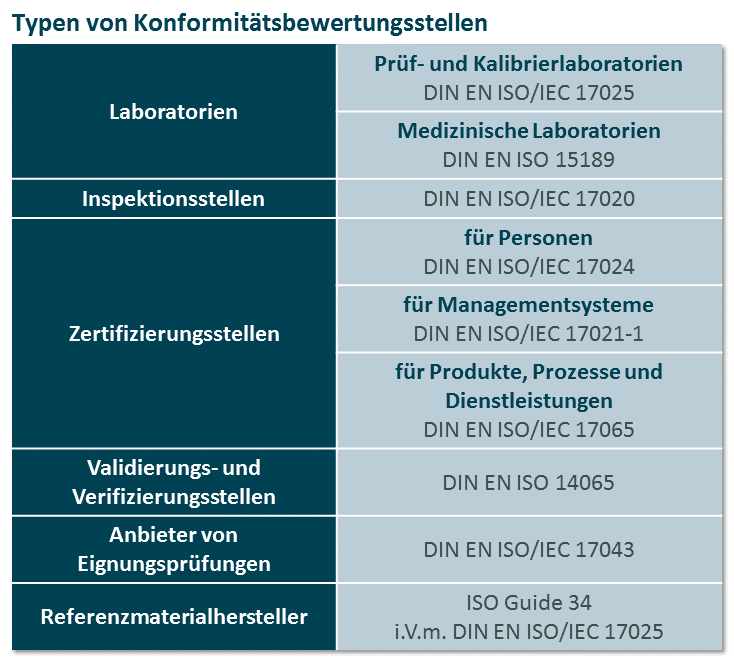
\includegraphics[width=120mm]{Bilder/TypenKBS.png}
		\caption{Typen von Konformitätsstellen, Quelle:\cite{DAkkS} }
		\label{fig:Typen_von_KBA}
	\end{center}
\end{figure}

Die internationale Harmonisierung dieser Normen gewährleistet, dass die Akkreditierung weltweit nach gleichen Voraussetzungen erfolgt. Durch diese harmonisierten Normen und dank internationaler Abkommen werden die Bewertungsleistungen der in Deutschland akkreditierten Stellen in vielen anderen Ländern Europas und der Welt anerkannt.

Diese Überwindung technischer Handelshemmnisse erleichtert den Handel über Grenzen hinweg und stellt sicher, dass die Ergebnisse von Konformitätsbewertungen ohne eine erneute Überprüfung \textit{international akzeptiert} werden.
\newpage
\textbf{Vorteile von Akkreditierungen}\newline
Für Unternehmen:
\begin{itemize}
\item Höhere Akzeptanz von Produkten und Dienstleistungen erleichtert den Marktzugang bzw. ermöglicht diesen erst
\item Einmal geprüft, überall akzeptiert: Internationale Vergleichbarkeit und Anerkennung von Zertifikaten, Inspektionen, Prüfungen oder Kalibrierungen vermeidet Kosten durch mehrfache Bewertungen
\item Kompetenznachweis erleichtert die Auswahl eines passenden Dienstleisters für die Konformitätsbewertung von Waren und Dienstleistungen
\end{itemize}
Für akkreditierte Stellen: 
\begin{itemize}
\item objektiver Beleg für die Güte und Kompetenz der Tätigkeit einer Konformitäts\-bewertungs\-stelle nach internationalen Standards
\item Wettbewerbsvorteile gegenüber nicht akkreditierten Marktteilnehmern
\end{itemize}
Für Verbraucher:
\begin{itemize}
\item größeres Vertrauen der Verbraucher in die Qualität von Produkten und Dienstleistungen – trotz eines komplexen Weltmarkts
\item weniger Produktfehler oder Rückrufaktionen
\end{itemize}
Für den Gesetzgeber: 
\begin{itemize}
\item verbesserte Wettbewerbsfähigkeit der Wirtschaft durch den Abbau \item technischer Handelshemnisse
\end{itemize}
\textbf{Akkreditierungsprozess}
\begin{itemize}
	
\item Antragsphase \newline
Der Akkreditierungsprozess beginnt mit der Einsendung des Akkreditierungsantrages und der fachspezifischen Anlagen an die Zentrale Antragsbearbeitung (ZAB) der DAkkS in Berlin.
Optional können sich Kunden auch vorab in einem Vorgespräch in den Geschäfts\-stel\-len der DAkkS über ihre angestrebte Akkreditierung oder das Akkreditierungsverfahren im konkreten Fall informieren.
Die ZAB überprüft in Abstimmung mit der zuständigen Fachabteilung der DAkkS den Antrag. Dabei wird auch geprüft, ob eine Befugnis erteilende Behörde (BeB) in das Akkreditierungsverfahren eingebunden werden muss.
Nach einer erfolgreichen Antragsprüfung informiert der zugeteilte Verfahrensmanager die antragstellende Konformitätsbewertungsstelle (KBS) über das weitere Vorgehen.

\item Begutachtungsphase \newline
In der zweiten Phase des Akkreditierungsprozesses begutachtet die DAkkS durch ein Begutachterteam die technische Kompetenz und das Managementsystem der KBS. Zunächst prüfen die Begutachter die eingereichten Dokumente, dann findet zum vereinbarten Termin die Begehung vor Ort statt. Der Umfang und die Dauer der Begutachtung sind von der Größe der KBS, dem beauftragten Geltungsbereich (Scope) der Akkreditierung und der Komplexität des Verfahrens abhängig.
Die Ergebnisse werden in einem Begutachtungsbericht dokumentiert.
Festgestellte Abweichungen kann der Kunde durch entsprechende Korrekturmaßnahmen im Anschluss an den Begutachtungstermin innerhalb von zwei Monaten beheben. Diese werden nochmals überprüft und bewertet.

\item Akkreditierungsphase \newline
In dieser Phase bewertet ein Akkreditierungsausschuss (AkA) die Begutachtungsergebnisse und entscheidet über die Erteilung der Akkreditierung.
Die DAkkS bescheinigt den erfolgreichen Abschluss der Akkreditierungsphase durch den Akkreditierungsbescheid und die Akkreditierungsurkunde. Damit bestätigt die DAkkS der überprüften KBS die Erfüllung der entsprechenden Normen, Standards oder Gesetzen im Hinblick auf ihre Konformitätbewertungstätigkeiten – und damit ihre technische Kompetenz.
Die Akkreditierung wird anschließend im Verzeichnis der akkreditierten Stellen gelistet.
\item Überwachungsphase \newline
Eine Akkreditierung ist in der Regel für fünf Jahre gültig. Um den Kompetenznachweis auch innerhalb dieser Zeit sicherzustellen, erfolgen in festgelegten Intervallen zwei bis drei Überwachungen – je nachdem, ob es sich um ein Laboratorium, eine Inspektions-, Zertifizierungs- oder Verifizierungsstelle handelt.
Der Akkreditierungszyklus endet spätestens nach fünf Jahren mit dem Auslaufen der Akkreditierung und bedarf dann einer Reakkreditierung.	
\end{itemize}
\textbf{Akkreditierungssymbol}\newline
Auf Antrag gestattet die DAkkS einer akkreditierten Stelle die Verwendung des DAkkS-Akkreditierungssymbols (siehe Abb.\ref{fig:SymbolDAkkS}). Zusammen mit der eindeutigen Registrierungsnummer weist es auf die erfolgreiche Akkreditierung hin. Durch die genehmigte Verwendung des Symbols können akkreditierte Stellen ihren Kunden die nachgewiesene Kompetenz signalisieren.
\begin{figure}[!htp]
	\begin{center}
		
\includegraphics[width=60mm]{Bilder/SymbolDAkkS.jpg}
		\caption{Muster des Akkreditierungssymbols der DAkkS für akkreditierte Stellen, Quelle:\cite{DAkkS} }
		\label{fig:SymbolDAkkS}
	\end{center}
\end{figure}

\textbf{Kosten der Akkreditierung} \newline
Als Deutschlands nationale Akkreditierungsstelle handelt die DAkkS zum Wohle des Staates, der Wirtschaft und der Verbraucher: Sie arbeitet im hoheitlichen Bereich kostendeckend, aber nicht gewinnorientiert.

\textbf{Gültigkeit von Akkreditierungen} \newline
Akkreditierungen sind üblicherweise fünf Jahre lang gültig, müssen jedoch in regelmäßigen Abständen durch die DAkkS überwacht werden.

\textbf{Änderungen in 2016: Eichbehören und PTB, 
DAkkS passt Regelung zur metrologischen Rückführung an}\newline
Die sogenannte „metrologische Rückführung“ ist eine der tragenden Säulen der Kon\-for\-mitäts\-bewertung. Die Deutsche Akkreditierungsstelle (DAkkS) hat ihre Regelungen zur Rück\-führungs\-politik nach Forderungen der Europäischen Kooperation für Akkreditierung (EA) angepasst. Danach ist ab August 2016 die Anerkennung von Rückführungsnachweisen, die von deutschen Eichbehörden ausgestellt wurden, nur noch in Einzelfällen möglich.Immer dann, wenn Messungen vorgenommen und die Messergebnisse für eine Kon\-formitäts\-bewert\-ung verwendet werden, ist die metrologische Rückführung von zentraler Bedeutung. Auf diesem Weg stellen Laboratorien und Inspektionsstellen die Richtigkeit der gemessenen Ergebnisse und der darauf basierenden Schlussfolgerungen – etwa die korrekte Einhaltung von Grenzwerten – sicher. Diese Stellen müssen daher im Rahmen eines Akkreditierungsverfahrens nachweisen, dass die Rückführung ihrer Messgeräte den internationalen Anforderungen entspricht.

Diese messtechnischen Anforderungen ergeben sich vor allem aus der Norm ISO/IEC 17025:2005 der Internationalen Organisation für Normung (ISO) sowie der verbindlichen Akkreditierungsregel ILAC P10:2013, die von der International Laboratory Accreditation Cooperation (ILAC) herausgegeben wird. Für alle durch die DAkkS akkreditierten Konformitätsbewertungsstellen sind diese Vorgaben in der DAkkS-Regel „Merkblatt zur messtechnischen Rückführung im Rahmen von Akkreditierungsverfahren“ (71 SD 0 005) zusammengefasst. Diese Regelung musste die DAkkS nun insbesondere im Hinblick auf die Rolle deutscher Eichbehörden anpassen.
In welchen Fällen sind Rückführungsnachweise deutscher Eichbehörden derzeit zulässig?

Die DAkkS-Regel 71 SD 0 005 zählt konkrete Möglichkeiten auf, wie Konformitätsbewertungsstellen gegenüber der DAkkS die Erfüllung der Anforderungen an die metrologische Rückführung nachweisen können. Eine bislang vorgesehene und praktizierte Möglichkeit bestand darin, einen Eichschein, Prüfschein oder Kalibrierschein einer deutschen Eichbehörde vorzulegen.

Voraussetzung dafür war bisher, dass die \textbf{ausstellende Eichbehörde} sich erfolgreich einem \textbf{Begutachtungsverfahren durch die Physikalisch-Technische Bundesanstalt (PTB), die metrologische Rückführung der relevanten Messgröße betreffend, unterzogen hat}. Dieses Vorgehen war aus Sicht der DAkkS, dem zuständigen Bundesministerium für Wirtschaft und Energie (BMWi) und der akkreditierten Konformitätsbewertungsstellen eine akzeptierte und praktikable Möglichkeit, den Nachweis der metrologischen Rückführung zu erbringen.

Warum wird sich die bisher gültige Regelung ändern?

Die europäische Akkreditierungsorganisation EA hat die Möglichkeit, Rückführungsnachweise von deutschen Eichbehörden unter gewissen Bedingungen zu akzeptieren, im Herbst 2014 bei der regelmäßig stattfindenden Evaluierung der DAkkS beanstandet, da Rückführungsnachweise ohne weitere Begutachtung durch die Akkreditierungsstelle nur dann anerkannt werden können, wenn die ausgebende Stelle den Rückführungsnachweis unter einer Akkreditierung erstellt hat. Eine Begutachtung durch die PTB allein ist hier nach dem internationalen Regelwerk (ISO/IEC 17025:2005) nicht ausreichend. Die DAkkS wurde im Oktober 2015 letztmalig aufgefordert, diese Regelung zu ändern.

EA hat diese Sichtweise am 28. Januar 2016 nochmals bestätigt, nachdem die DAkkS dagegen ein zulässiges Beschwerdeverfahren eingeleitet hatte. Als Folge dieser EA-Entscheidung hat die DAkkS in Abstimmung mit dem BMWi und der PTB die DAkkS-Regel 71 SD 0 005 überarbeitet und in der Revision 1.4 am 1. Februar 2016 veröffentlicht.

\subsection{Zertifizierung}

Als \glqq Zertifizierung \grqq~ (von lat. \glqq certe\grqq~ = bestimmt, gewiss, sicher und „facere“ = machen, schaffen, verfertigen) bezeichnet man ein Verfahren, mit dessen Hilfe die Einhaltung bestimmter Anforderungen nachgewiesen wird.

Zertifizierung ist ein Teilprozess der Konformitätsbewertung. Zertifizierungen werden oft zeitlich befristet von unabhängigen Zertifizierungsstellen wie z. B. DQS, TÜV oder DEKRA vergeben und die Standards unabhängig kontrolliert.

Anforderungsbereiche\newline
Die Bereiche, in denen Anforderungen gestellt werden, die zertifiziert werden können, umfassen im Allgemeinen:
\begin{itemize}
\item Produkte und Dienstleistungen und ihre jeweiligen Herstellungsverfahren einschließlich der Handelsbeziehungen
\item Personen
\item Systeme
\item Unternehmen
\end{itemize}

\textbf{Arten der Zertifizierung }
\begin{itemize}
\item Nachweis von Ausbildungsstandards oder besonders ausgearbeiteten Fachnormen bei Personenzertifizierungen. 
\item Nachweis von Ausbildungsstandards bei der Anerkennung von Ausbildungsinstituten, wie er beispielsweise durch Berufsverband|Berufsverbände durchgeführt wird (bei nichtuniversitären Ausbildungen wird teils von \glqq zertifizierten\grqq ~Ausbildungsinstituten, teils von \glqq akkreditierten\grqq ~Ausbildungsinstituten gesprochen, wobei Letztere zugleich befugt sind, Personenzertifikationen oder Teile davon durchzuführen).
\item International anerkannter Nachweis der persönlichen Befähigung, zum Beispiel als PMP (Project Management Professional) durch das PMI (Project Management Institute) IPMA-Zertifikate Level D-A für Projektmanager.
\item Zertifizierung eines Managementsystems (zum Beispiel nach ISO 9001, ISO 14001). 
\item Zertifizierung von Produkten oder Dienstleistungen. Für Zertifizierungsstellen, die Zertifizierungssysteme für Produkte oder Dienstleistungen betreiben, besteht die EN ISO/IEC 17065 (früher EN 45011 bzw. ISO/IEC Guide 65).
\item Zertifizierung der Herkunftsregion eines Produktes (DOC).
\item Zertifizierung der Informationssicherheit nach BS 7799 oder ISO 27001|ISO/IEC 27001.
\item Zertifizierung zum Nachweis der Einhaltung von Umwelt- und Sozialstandards, zum Beispiel bei der Zertifizierung von nachhaltig erzeugtem Holz (siehe Zertifizierung (Forstwirtschaft)|FSC) oder von Produkten aus Entwicklungsländern, die bessere Konditionen für die dortigen Produzenten garantieren nach Fairer Handel|Fair-Trade-Kriterien.
\item Zertifizierung zum Nachweis der Einhaltung von Anforderungen an den Arbeitssicherheit, Arbeits- und Umweltschutz gem. Occupational Safety and Health Administration|OHSAS bzw. ISO 14001
\item Zertifizierung zum Nachweis von Arbeitsbedingungen gemäß SA8000 und ähnlichen Regelwerken (Beispiele: Sedex und Business Social Compliance Initiative|BSCI).
\item In der Software-Industrie ist die Zertifizierung insbesondere im Hinblick auf die Computersicherheit wichtig:
\item Zertifizierung der Mitarbeiter zur Dokumentation von Fähigkeiten, Qualifikation und Kompetenz. Siehe dazu Liste der IT-Zertifikate.
\item Zertifizierung von Softwareprodukten in Hinblick auf Funktionalität und Qualität. Besonders wichtig sind hier der amerikanische TCSEC- und der Europäische Information Technology Security Evaluation Criteria-Standard sowie im Hinblick auf die internationale Anerkennung die Common Criteria (CC). In Deutschland erfolgt die Zertifizierung durch das Bundesamt für Sicherheit in der Informationstechnik|BSI.
\item Zertifizierung der IT-Umgebung nach IT-Grundschutz. Um in einem Unternehmen einen solchen Prozess zu begleiten, werden vom BSI Grundschutz-Auditoren lizenziert. Diese sind autorisiert, Testate als Vorbereitung auf die Zertifizierung auszugeben. Die eigentliche Zertifizierung erfolgt durch das BSI.
\item Im Bereich Linux und freie Software ist ein wichtiges zertifizierendes Institut das kanadische Linux Professional Institute|LPI.
\item In der Lebensmittelindustrie gibt es heute verschiedene Normen, angelehnt an die weltweit bekannte ISO 9001. Diese wurden zugeschnitten auf die Bedürfnisse der Lebensmittelindustrie. Weit verbreitete Standards sind zum Beispiel der International Food Standard (IFS), die Anforderungen des British Retail Consortium, Good Manufacturing Practice|GMP, Hazard Analysis and Critical Control Points und die ISO 22000. Zunehmender Akzeptanz erfreut sich für Fische auch der MSC-Standard des Marine Stewardship Council.
\item Packmittelhersteller, die Packmittel für den direkten Kontakt mit Lebensmitteln (Pri\-mär\-pack\-mit\-tel) herstellen, sind zunehmend nach der Norm BRC-IoP zertifiziert.
\item Zertifizierung von Altersvorsorgeprodukten, z. B. Riesterrente.
\item Zertifizierung von Energiemanagementsystemen gemäß ISO 50001.
\item Nachhaltigkeitszertifizierung von Biomasse und Biokraftstoffen.
\item Unternehmenszertifizierung, z.B. für den Bereich Nachhaltigkeit. Hier werden Standards vom Standardgeber vorgeschrieben. In diesem Fall wird vom Standardgeber definiert, was Nachhaltigkeit im unternehmerischen Kontext bedeutet. Das gesamte Unternehmen (Management, Lieferketten, Produkte usw.) wird im Zertifizierungsprozess überprüft.
\end{itemize}

\subsection{Konfirmitätsbewertung}
\glqq Konformitätsbewertung\grqq~ist in der internationalen Norm ISO/IEC 17000:2004 \glqq Kon\-for\-mitäts\-be\-wertung – Begriffe und allgemeine Grundlagen\grqq definiert als \glqq Darlegung, dass festgelegte Anforderungen bezogen auf ein Produkt, einen Prozess, ein System, eine Person oder eine Stelle erfüllt sind\grqq.

Konformitätsbewertung ist ein Überbegriff für Tätigkeiten des Auswählens, Ermittelns (von Eigenschaften), Bewertens (etwa auf Einhaltung vorgegebener oder allgemeiner Anforderungen) und Bestätigens (etwa durch Konformitätserklärung|Erklärung des Herstellers, oder ein Zertifizierung|Zertifikat einer Zertifizierungsstelle, dass ein Produkt bestimmte Normen einhält). Solche Tätigkeiten sind beispielsweise Stichprobennahme, Prüfen, Inspizieren, Erklären, Zertifizieren, Akkreditieren. Die Objekte der Konformitätsbewertung sind nicht eingeschränkt.

Konformitätsbewertung findet auf vielfältige Weise und allen Ebenen statt: 
\begin{itemize}
\item im Betrieb (etwa Endprüfung, Auditierung eines Qualitätsmanagementsystems durch eigene Auditoren):
\item durch Stellen / Personen des Kunden oder Abnehmers: 
\item durch kommerzielle, vom Auftraggeber unabhängige Konformitätsbewertungsstellen (etwa Laboratorien; Zertifizierungsstellen; Inspektionsstellen; Akkreditierung (Wirtschaft), Akkreditierungsstellen): 
\end{itemize}

EU-Konformitätsbewertung

Eine besondere Bedeutung hat die Konformitätsbewertung durch Benannte Stellen bei der Bewertung von Produkten auf ihre Übereinstimmung mit den Anforderungen einer Richtlinie (EU)|EU-Richtlinie. EU-Richtlinien gemäß Art. 95 EG-Vertrag für den Europäischer Binnenmarkt|Europäischen Binnenmarkt legen für zahlreiche Produkte Mindestanforderungen an die Sicherheit fest, die vom Hersteller erfüllt werden müssen.

Durch ein \glqq Konformitätsbewertungsverfahren\grqq~muss der Hersteller nachweisen, dass er die in der Richtlinie oder den Richtlinien enthaltenen grundlegenden Sicherheitsanforderungen eingehalten hat. Das Konformitätsbewertungsverfahren muss vom Hersteller für jedes Produkt vor dem erstmaligen Inverkehrbringen durchgeführt werden. Am Ende des Kon\-formitäts\-bewertungs\-verfahrens stellt der Hersteller eine EU-Konformitätserklärung für sein Produkt aus, in der er erklärt, dass das Produkt zu den Anforderungen der entsprechenden Richtlinie(n) konform ist. Am Produkt bringt der Hersteller dann die CE-Kennzeichnung an, falls die angewandte Richtlinie dies vorsieht.

Nur im Sektor \glqq Medizinprodukte\grqq~besteht die Besonderheit, dass im Rahmen der Konformitätsbewertung nicht nur die Produktsicherheit nachgewiesen werden muss, sondern zusätzlich auch die medizinisch-technische Leistungsfähigkeit von Medizinprodukten, so wie sie vom Hersteller in der Produktkennzeichnung einschließlich der Werbung als medizinische Indikation ausgelobt ist. Das entsprechende Nachweisverfahren nennt sich klinische Bewertung. Erst der (je nach der Produktklasse) extern durch Benannte Stelle zertifizierte Nachweis der Produktsicherheit und der Leistungsfähigkeit berechtigt Hersteller von Medizinprodukten zur Anbringung der \textbf{CE-Kennzeichnung}.

In den Anhängen der Richtlinien werden verschiedene Module für die Durchführung eines Konformitätsbewertungsverfahrens genannt. Welche Module gewählt werden können, hängt von der Klassifizierung des Produktes ab. Für Produkte mit höherem Risiko ist die Einbeziehung einer Benannten Stelle bei der Durchführung des Konformitätsbewertungsverfahrens obligatorisch.
Beispiele für Module:
\begin{itemize}
\item Modul A2: Interne Fertigungskontrolle durch den Hersteller und Überwachung der Abnahme durch benannte Stelle 
\item Modul B \textit{Baumusterprüfung}
EG-Baumusterprüfung (Feststellung der Übereinstimmung mit den einschlägigen internationalen und nationalen Fachnormen (DIN, EN, ISO, IEC etc.), IMO-Resolutionen und SOLAS-Bestimmungen)
\item Modul D
: Qualitätssicherung Produktion (Darlegung der Qualitätssicherungsmaßnahmen vor, während und nach der Produktion einschließlich deren Häufigkeit)
\item Modul E
: Qualitätssicherung Produkt (Darlegung der Qualitätssicherungsmaßnahmen nach der Produktion einschließlich deren Häufigkeit (Endabnahme und Prüfung))
\item Modul F
: Prüfung der Produkte (Prüfung der Produkte auf Übereinstimmung mit dem Baumuster entweder durch statistische Kontrollen oder Prüfung jedes einzelnen Produkts durch die Benannte Stelle)
\item Modul G
: Einzelprüfung (anwendbar auf Produkte, die nicht in Serie produziert werden)
\end{itemize}
Je höher das Gefahrenpotential eines Produktes ist, umso mehr Prüfungsumfang muss auf eine „Benannte Stelle“ übertragen werden. Diese wird durch eine vierstellige Kennziffer hinter der CE-Kennzeichnung angegeben. Die Konformitätsbewertung für Produkte mit einem sehr geringen Gefährdungspotenzial kann der Hersteller ohne Einschaltung einer Benannten Stelle selbst durchführen.

In jedem Fall - also auch bei Einschaltung einer Drittstelle - muss eine EU-Konformitätserklärung (in der Regel) durch den Hersteller ausgestellt werden. Dies unterstreicht dessen alleinige Verantwortung (= Haftung) für das Produkt.

Bei der Konformitätsbewertung müssen die Sicherheitsanforderungen der EU-Richtlinien eingehalten werden. 

\subsection{Audit}
Ein \glqq Audit\grqq~untersucht, ob Geschäftsprozesse, Anforderungen und Richtlinien die geforderten Standards erfüllen. Ein solches Untersuchungsverfahren erfolgt häufig im Rahmen eines Qualitätsmanagements. Die Audits werden von einem speziell hierfür geschulten Auditor durchgeführt.

Innerhalb des Qualitätsmanagements werden zwei Arten von Audits unterschieden: Im Bereich des Qualitätssicherung, statischen Qualitätsmanagements haben die Audits Prüfungscharakter, da sie  Nachweise über vertragsmäßige Vereinbarungen liefern. Sie werden daher pro Über\-prüfungs\-zyklus nur einmalig durchgeführt. In der Qualitätssicherung, dynamischen Qualitäts\-sicherung (oder Qualitätsmanagement) kommt den Audits eine erweiterte Bedeutung zu: Sie dienen der Erfassung von Entwicklungstrends und geben den Initiatoren von Veränderungen wichtige Rückmeldungen über die Wirksamkeit ihrer eingeleiteten Maßnahmen. Die Aussagekraft dieser begleitenden Audits steigt mit der Wiederholungsrate, mit der der identische Fragenkatalog der identischen Betroffenengruppe zum identischen Thema vorgelegt wird. Vorgaben macht die \glqq DIN/ISO 19011, Leitfaden zur Auditierung von Managementsystemen\grqq.

\subsection{DAkkS}
Wie bereits oben erwähnt ist die 
die \glqq Deutsche Akkreditierungsstelle GmbH\grqq ~(\glqq DAkkS\grqq) zuständig für Akkreditierungen. Sie ist die nationale Akkreditierungsstelle mit Sitz in Berlin.

Gründungsgeschichte \newline
Im Zuge der europäischen Verordnung (EG) Nr. 765/2008 (Artikel 4 Absatz 1) müssen alle EU-Mitgliedstaaten ab 1. Januar 2010 eine einzige nationale Akkreditierungsstelle benennen. Hierzu musste die Dachorganisation Deutscher Akkreditierungsrat (DAR) mit den folgenden vier Fachgesellschaften für bestimmte Gebiete zur DAkkS fusionieren:
\begin{itemize}
\item Deutsche Akkreditierungsstelle Chemie (DACH)
\item Deutscher Kalibrierdienst (DKD)
\item Deutsches Akkreditierungssystem Prüfwesen (DAP)
\item Trägergemeinschaft für Akkreditierung (TGA)
Über eine vorweggenommene Fusion enthält die TGA auch die Deutsche Akkreditierungsstelle Technik (DATech)
\end{itemize}
Organisation \newline
Die DAkkS ist eine privatwirtschaftliche Organisation, beliehene hoheitliche Aufgaben wahrnimmt. 

Die GmbH-Anteilseigner der DAkkS sind jeweils zu einem Drittel:
\begin{itemize}
\item die Bundesländer, vertreten durch die Länder Bayern, Hamburg, Niedersachsen, Nordrhein-Westfalen und Sachsen-Anhalt. 
\item die Bundesrepublik Deutschland, vertretend durch das Bundesministerium für Wirtschaft und Energie 
\item die Deutsche Wirtschaft, vertretend durch den Bundesverband der Deutschen Industrie (BDI). 
\end{itemize}
Die Bundesländer wurden primär beteiligt, um die bestehenden Organisationen der Länder leichter in die DAkkS zu überführen, \glqq wodurch parallele Strukturen und Aktivitäten auf Landesebene verzichtbar werden\grqq.

Kritik an der DAkkS: \textit{In einer gemeinsamen Erklärung kritisierten Eurolab-D, der Verband der Materialprüfungsanstalten (VMPA) e.V. und der Deutsche Verband Unabhängiger Prüf\-labor\-atorien (VUP) die vom Bundeswirtschaftsministerium (BMWi) vorgelegte Reform der Gebührenverordnung für die Akkreditierungsstelle. Die Preissteigerungsrate schade dem Mittelstand und somit dem Wirtschaftsstandort Deutschland.}

\end{comment}
\newpage
% % Die neue Fassung der weltweit gültigen Norm ISO/IEC 17025 für Laborakkreditierungen ist Ende November in englischer Fassung
% erschienen und enthält viele grundlegende Änderungen.  
% \section*{Anhang}
% \subsection*{A1: Herleitung }

% \newpage
% \section*{Übungsaufgaben}
